% diag_architecture: TikZ twin of paper/figures/diag_architecture.pdf (generated by diag_common.py).
% Coordinates are inches (y up). Needs \usepackage{tikz}. Body font 7 pt.
\definecolor{dgA}{HTML}{F0F0F0}\definecolor{dgB}{HTML}{DCDCDC}\definecolor{dgC}{HTML}{C4C4C4}
\definecolor{dgAtk}{HTML}{F2C9B8}\definecolor{dgHw}{HTML}{E3EEF7}
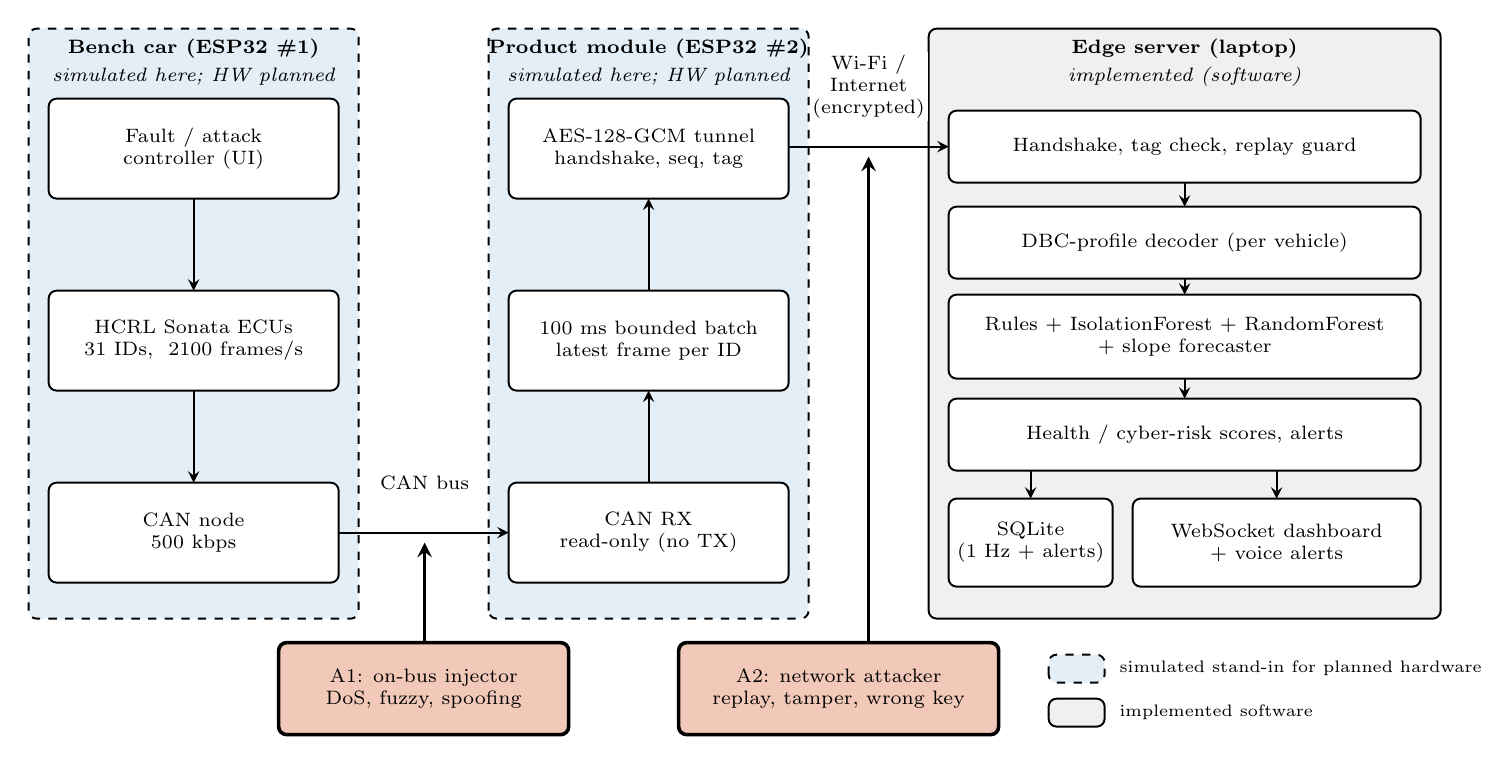
\begin{tikzpicture}[x=1in,y=1in,>=stealth,font=\fontsize{7}{8}\selectfont,line width=0.7pt]
\draw[rounded corners=2.9pt,fill=dgHw,line width=0.7pt,dashed] (0.050,0.620) rectangle (1.700,3.570);
\node[align=center,inner sep=0pt] at (0.875,3.470) {\bfseries \fontsize{7.0}{7.8}\selectfont Bench car (ESP32 \#1)};
\node[align=center,inner sep=0pt] at (0.875,3.330) {\itshape \fontsize{6.8}{7.6}\selectfont simulated here; HW planned};
\draw[rounded corners=2.9pt,fill=dgHw,line width=0.7pt,dashed] (2.350,0.620) rectangle (3.950,3.570);
\node[align=center,inner sep=0pt] at (3.150,3.470) {\bfseries \fontsize{7.0}{7.8}\selectfont Product module (ESP32 \#2)};
\node[align=center,inner sep=0pt] at (3.150,3.330) {\itshape \fontsize{6.8}{7.6}\selectfont simulated here; HW planned};
\draw[rounded corners=2.9pt,fill=dgA,line width=0.7pt] (4.550,0.620) rectangle (7.110,3.570);
\node[align=center,inner sep=0pt] at (5.830,3.470) {\bfseries \fontsize{7.0}{7.8}\selectfont Edge server (laptop)};
\node[align=center,inner sep=0pt] at (5.830,3.330) {\itshape \fontsize{6.8}{7.6}\selectfont implemented (software)};
\draw[rounded corners=2.9pt,fill=white,line width=0.7pt] (0.150,2.720) rectangle (1.600,3.220);
\node[align=center,inner sep=0pt] at (0.875,2.970) {\fontsize{7.0}{7.8}\selectfont Fault / attack\\ controller (UI)};
\draw[rounded corners=2.9pt,fill=white,line width=0.7pt] (0.150,1.760) rectangle (1.600,2.260);
\node[align=center,inner sep=0pt] at (0.875,2.010) {\fontsize{7.0}{7.8}\selectfont HCRL Sonata ECUs\\ 31 IDs, ~2100 frames/s};
\draw[rounded corners=2.9pt,fill=white,line width=0.7pt] (0.150,0.800) rectangle (1.600,1.300);
\node[align=center,inner sep=0pt] at (0.875,1.050) {\fontsize{7.0}{7.8}\selectfont CAN node\\ 500 kbps};
\draw[->,line width=0.8pt] (0.875,2.720) -- (0.875,2.260);
\draw[->,line width=0.8pt] (0.875,1.760) -- (0.875,1.300);
\draw[->,line width=0.8pt] (1.600,1.050) -- (2.450,1.050);
\node[align=center,fill=white,inner sep=1pt] at (2.030,1.300) {\fontsize{6.8}{7.6}\selectfont CAN bus};
\draw[rounded corners=2.9pt,fill=dgAtk,line width=1.3pt] (1.300,0.040) rectangle (2.750,0.500);
\node[align=center,inner sep=0pt] at (2.025,0.270) {\fontsize{7.0}{7.8}\selectfont A1: on-bus injector\\ DoS, fuzzy, spoofing};
\draw[->,line width=1.3pt] (2.030,0.500) -- (2.030,1.000);
\draw[rounded corners=2.9pt,fill=white,line width=0.7pt] (2.450,2.720) rectangle (3.850,3.220);
\node[align=center,inner sep=0pt] at (3.150,2.970) {\fontsize{7.0}{7.8}\selectfont AES-128-GCM tunnel\\ handshake, seq, tag};
\draw[rounded corners=2.9pt,fill=white,line width=0.7pt] (2.450,1.760) rectangle (3.850,2.260);
\node[align=center,inner sep=0pt] at (3.150,2.010) {\fontsize{7.0}{7.8}\selectfont 100 ms bounded batch\\ latest frame per ID};
\draw[rounded corners=2.9pt,fill=white,line width=0.7pt] (2.450,0.800) rectangle (3.850,1.300);
\node[align=center,inner sep=0pt] at (3.150,1.050) {\fontsize{7.0}{7.8}\selectfont CAN RX\\ read-only (no TX)};
\draw[->,line width=0.8pt] (3.150,1.300) -- (3.150,1.760);
\draw[->,line width=0.8pt] (3.150,2.260) -- (3.150,2.720);
\draw[->,line width=0.8pt] (3.850,2.980) -- (4.650,2.980);
\node[align=center,fill=white,inner sep=1pt] at (4.250,3.280) {\fontsize{6.8}{7.6}\selectfont Wi-Fi /\\ Internet\\ (encrypted)};
\draw[rounded corners=2.9pt,fill=dgAtk,line width=1.3pt] (3.300,0.040) rectangle (4.900,0.500);
\node[align=center,inner sep=0pt] at (4.100,0.270) {\fontsize{7.0}{7.8}\selectfont A2: network attacker\\ replay, tamper, wrong key};
\draw[->,line width=1.3pt] (4.250,0.500) -- (4.250,2.930);
\draw[rounded corners=2.9pt,fill=white,line width=0.7pt] (4.650,2.800) rectangle (7.010,3.160);
\node[align=center,inner sep=0pt] at (5.830,2.980) {\fontsize{7.0}{7.8}\selectfont Handshake, tag check, replay guard};
\draw[rounded corners=2.9pt,fill=white,line width=0.7pt] (4.650,2.320) rectangle (7.010,2.680);
\node[align=center,inner sep=0pt] at (5.830,2.500) {\fontsize{7.0}{7.8}\selectfont DBC-profile decoder (per vehicle)};
\draw[rounded corners=2.9pt,fill=white,line width=0.7pt] (4.650,1.820) rectangle (7.010,2.240);
\node[align=center,inner sep=0pt] at (5.830,2.030) {\fontsize{7.0}{7.8}\selectfont Rules + IsolationForest + RandomForest\\ + slope forecaster};
\draw[rounded corners=2.9pt,fill=white,line width=0.7pt] (4.650,1.360) rectangle (7.010,1.720);
\node[align=center,inner sep=0pt] at (5.830,1.540) {\fontsize{7.0}{7.8}\selectfont Health / cyber-risk scores, alerts};
\draw[rounded corners=2.9pt,fill=white,line width=0.7pt] (4.650,0.780) rectangle (5.470,1.220);
\node[align=center,inner sep=0pt] at (5.060,1.000) {\fontsize{6.8}{7.6}\selectfont SQLite\\ (1 Hz + alerts)};
\draw[rounded corners=2.9pt,fill=white,line width=0.7pt] (5.570,0.780) rectangle (7.010,1.220);
\node[align=center,inner sep=0pt] at (6.290,1.000) {\fontsize{6.8}{7.6}\selectfont WebSocket dashboard\\ + voice alerts};
\draw[->,line width=0.8pt] (5.830,2.800) -- (5.830,2.680);
\draw[->,line width=0.8pt] (5.830,2.320) -- (5.830,2.240);
\draw[->,line width=0.8pt] (5.830,1.820) -- (5.830,1.720);
\draw[->,line width=0.8pt] (5.060,1.360) -- (5.060,1.220);
\draw[->,line width=0.8pt] (6.290,1.360) -- (6.290,1.220);
\draw[rounded corners=2.9pt,fill=dgHw,line width=0.7pt,dashed] (5.150,0.300) rectangle (5.430,0.440);
\node[anchor=west,align=flush left,inner sep=0pt] at (5.500,0.370) {\fontsize{6.5}{7.3}\selectfont simulated stand-in for planned hardware};
\draw[rounded corners=2.9pt,fill=dgA,line width=0.7pt] (5.150,0.080) rectangle (5.430,0.220);
\node[anchor=west,align=flush left,inner sep=0pt] at (5.500,0.150) {\fontsize{6.5}{7.3}\selectfont implemented software};
\end{tikzpicture}
